% This is samplepaper.tex, a sample chapter demonstrating the
% LLNCS macro package for Springer Computer Science proceedings;
% Version 2.21 of 2022/01/12
%
\documentclass[runningheads]{llncs}
%
\usepackage{tikz}
\usepackage[T1]{fontenc}
% T1 fonts will be used to generate the final print and online PDFs,
% so please use T1 fonts in your manuscript whenever possible.
% Other font encondings may result in incorrect characters.
%
\usepackage{graphicx}
% Used for displaying a sample figure. If possible, figure files should
% be included in EPS format.
%
% If you use the hyperref package, please uncomment the following two lines
% to display URLs in blue roman font according to Springer's eBook style:
%\usepackage{color}
%\renewcommand\UrlFont{\color{blue}\rmfamily}
%\urlstyle{rm}
%
\begin{document}
%
\title{Contribution Title}
%
%\titlerunning{Abbreviated paper title}
% If the paper title is too long for the running head, you can set
% an abbreviated paper title here
%
\author{First Author\inst{1}\orcidID{0000-1111-2222-3333} \and
Second Author\inst{2,3}\orcidID{1111-2222-3333-4444} \and
Third Author\inst{3}\orcidID{2222--3333-4444-5555}}
%
\authorrunning{F. Author et al.}
% First names are abbreviated in the running head.
% If there are more than two authors, 'et al.' is used.
%
\institute{Princeton University, Princeton NJ 08544, USA \and
Springer Heidelberg, Tiergartenstr. 17, 69121 Heidelberg, Germany
\email{lncs@springer.com}\\
\url{http://www.springer.com/gp/computer-science/lncs} \and
ABC Institute, Rupert-Karls-University Heidelberg, Heidelberg, Germany\\
\email{\{abc,lncs\}@uni-heidelberg.de}}
%
\maketitle              % typeset the header of the contribution
%
\begin{abstract}
Tableux proof are used in automated  "proofers" as (TODO), wereas sequent calculus 
proofs are used in proof assitants as (TODO). This work aims to present a systematic 
algorithm for translating tableaux proofs into sequent calculus proofs.
It begins with an overview of the definitions underlying such translations 
in both intuitionistic and classical logic.
 It then shows a translation process in classical logic, along with its properties. 
 Finally, potential extensions toward translations in intuitionistic logic are explored.
\keywords{Tableux proof  \and  sequent calculus  \and intuitionistic logic.}
\end{abstract}
%
%
%
\section{Underlying concepts}
%(TODO how detailed? < or > than thepresentation? )
The sintax and semantics from both classical and intuitionistic logic is based on \cite{book2}. 
In this work, sentences wont have function symbols.
\subsection{Language}
\begin{definition}
\item A \textbf{Language} $\mathcal{L}$ is a set of symbols, including:
\begin{itemize}
    \item parentheses $($ and $)$ 
    \item logical connectives $\neg,\land,\lor,\to$
    \item variable symbols $x,y,z,\ldots$
    \item constant symbols $c_{1},c_{2},\ldots$
   (% \item function symbols $p,q,r,\ldots$ %)
    \item quantifier symbols $\forall,\exists$
    \item predicate symbols $P,Q,R,\ldots$
\end{itemize}

\end{definition}

()Every predicate is a formula, and if \a


()Sentences 


()Signed sentences
\subsection{Truth in classical logic}


\subsection{Truth in intuitionistic logic}


\subsubsection{Kripke structures} 

\begin{definition}
    A kripke structure is a s
\end{definition}

\subsubsection{Kripke Frames} 
\begin{definition}
    Kripe 
\end{definition}

\subsection{Translation in classical logic}
    We first define a slightly diferent version of a tableaux proof tree \cite{book1}, 
    were each node is represented by a set of signed sentences. Intuitively, 
    a node in the usal definiton is replaced by set of 
    all nodes in the path that goes from the root to him. %[TODO "root to him" is a bit ugly]  

    A tree with a single node $\{F \phi \}$ is a tableaux development of $\phi$. 
    Given a signed sentence $\sigma$ in a leaf $\{T \Gamma_1, T\Gamma_2, \ldots, F \Delta_1, F \Delta_2, \ldots\}$ of a
    tableaux development $\tau$ of $\phi$, we define : 
    $\f(\sigma,\tau)$:
    \begin{itemize}
        \item $\hookrightarrow(T \neg \alpha,\tau) = \tau$ with $L \cup \{F \alpha\}$ 
        added (adjoined?) to all leaves $L$ that contain $T \neg \alpha$.
        \item $f(F \neg \alpha,\tau) = \tau$ with $L \cup \{T \alpha\}$ 
        added (adjoined?) to all leaves $L$ that contain $F \neg \alpha$.
        \item $f(T (\alpha \land \beta),\tau) = \tau$ with $L \cup \{T \alpha, T \beta\}$ 
        added to all leaves $L$ that contain $T (\alpha \land \beta)$.
        \item $f(F (\alpha \land \beta),\tau) = \tau$ with $L \cup \{F \alpha\}$ and $L \cup \{F \beta\}$ 
        added to all leaves $L$ that contain $F (\alpha \land \beta)$.
        \item $f(T (\alpha \lor \beta),\tau) = \tau$ with $L \cup \{T \alpha\}$ and $L \cup \{T \beta\}$ 
        added to all leaves $L$ that contain $T (\alpha \lor \beta)$.
        \item $f(F (\alpha \lor \beta),\tau) = \tau$ with $L \cup \{F \alpha, F \beta\}$ 
        added to all leaves $L$ that contain $F (\alpha \lor \beta)$.
        \item $f(T (\alpha \to \beta),\tau) = \tau$ with $L \cup \{F \alpha\}$ and $L \cup \{T \beta\}$ 
        added to all leaves $L$ that contain $T (\alpha \to \beta)$.
        \item $f(F (\alpha \to \beta),\tau) = \tau$ with $L \cup \{T \alpha, F \beta\}$ 
        added to all leaves $L$ that contain $F (\alpha \to \beta)$.
     \end{itemize}


     A tree with a single node $\{F \phi \}$ is a tableaux development of $\phi$. 
    Given a signed sentence $\sigma$ in a leaf $\{T \Gamma_1, T\Gamma_2, \ldots, F \Delta_1, F \Delta_2, \ldots\}$ of a
    tableaux development $\tau$ of $\phi$, we denote $\tau \hookrightarrow_{\sigma} \tau'$
    as a function that takes a tableaux development of phi and gives another tree. 
    \begin{center}
        \begin{scriptsize}
        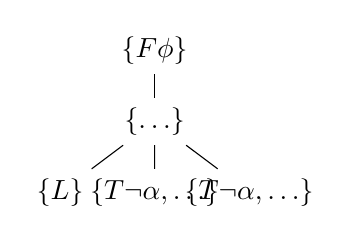
\begin{tikzpicture}[scale=0.6
            , level distance=1.5cm,
            level 1/.style={sibling distance=3cm},
            level 2/.style={sibling distance=2cm}]
        \node {$\{F \phi\}$}
            child {node {$\{\ldots\}$}
                child {node {$\{L\}$}}
                child {node {$\{T \neg \alpha, \ldots\}$}}
                child {node {$\{T \neg \alpha, \ldots\}$}}
            };
        \end{tikzpicture}
        \hspace{1.5cm} $\hookrightarrow$ \hspace{1.5cm}
        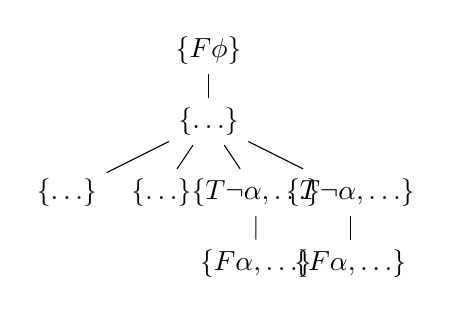
\begin{tikzpicture}[scale=0.6, level distance=1.5cm,
            level 1/.style={sibling distance=3cm},
            level 2/.style={sibling distance=2cm}]
        \node {$\{F \phi\}$}
            child {node {$\{\ldots\}$}
                child {node {$\{\ldots\}$}}
                child {node {$\{\ldots\}$}}
                child {node {$\{T \neg \alpha, \ldots\}$}
                    child {node {$\{F \alpha, \ldots\}$}}}
                child {node {$\{T \neg \alpha, \ldots\}$}
                    child {node {$\{F \alpha, \ldots\}$}}}
            };
        \end{tikzpicture}
        \end{scriptsize}
    \end{center}


    \begin{center}
        \begin{tikzpicture}[level distance=2cm,
            level 1/.style={sibling distance=4cm},
        \node {$\{T \neg \alpha, \ldots\}$}

        \end{tikzpicture}
    \end{center}

    \begin{center}
    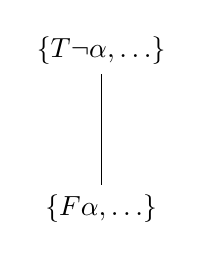
\begin{tikzpicture}[level distance=2cm,
        level 1/.style={sibling distance=4cm},
        level 2/.style={sibling distance=2cm}]
    \node {$\{T \neg \alpha, \ldots\}$}
            child {node {$\{F \alpha, \ldots\}$}};
    \end{tikzpicture}
    \end{center}



    Definition: f($\tau$,$\phi$) is tableaux development of $\phi$.
 


\begin{table}
\caption{Table captions should be placed above the
tables.}\label{tab1}
\begin{tabular}{|l|l|l|}
\hline
Heading level &  Example & Font size and style\\
\hline
Title (centered) &  {\Large\bfseries Lecture Notes} & 14 point, bold\\
1st-level heading &  {\large\bfseries 1 Introduction} & 12 point, bold\\
2nd-level heading & {\bfseries 2.1 Printing Area} & 10 point, bold\\
3rd-level heading & {\bfseries Run-in Heading in Bold.} Text follows & 10 point, bold\\
4th-level heading & {\itshape Lowest Level Heading.} Text follows & 10 point, italic\\
\hline
\end{tabular}
\end{table}


\noindent Displayed equations are centered and set on a separate
line.
\begin{equation}
x + y = z
\end{equation}
Please try to avoid rasterized images for line-art diagrams and
schemas. Whenever possible, use vector graphics instead (see
Fig.~\ref{fig1}).

\begin{figure}
\includegraphics[width=\textwidth]b.png}
\caption{A figure caption is always placed below the illustration.
Please note that short captions are centered, while long ones are
justified by the macro package automatically.} \label{fig1}
\end{figure}

\begin{theorem}
This is a sample theorem. The run-in heading is set in bold, while
the following text appears in italics. Definitions, lemmas,
propositions, and corollaries are styled the same way.
\end{theorem}
%
% the environments 'definition', 'lemma', 'proposition', 'corollary',
% 'remark', and 'example' are defined in the LLNCS documentclass as well.
%
\begin{proof}
Proofs, examples, and remarks have the initial word in italics,
while the following text appears in normal font.
\end{proof}
For citations of references, we prefer the use of square brackets
and consecutive numbers. Citations using labels or the author/year
convention are also acceptable. The following bibliography provides
a sample reference list with entries for journal
articles~\cite{ref_article1}, an LNCS chapter~\cite{ref_lncs1}, a
book~\cite{ref_book1}, proceedings without editors~\cite{ref_proc1},
and a homepage~\cite{ref_url1}. Multiple citations are grouped
\cite{ref_article1,ref_lncs1,ref_book1},
\cite{ref_article1,ref_book1,ref_proc1,ref_url1}.

\begin{credits}
\subsubsection{\ackname} A bold run-in heading in small font size at the end of the paper is
used for general acknowledgments, for example: This study was funded
by X (grant number Y).

\subsubsection{\discintname}
It is now necessary to declare any competing interests or to specifically
state that the authors have no competing interests. Please place the
statement with a bold run-in heading in small font size beneath the
(optional) acknowledgments\footnote{If EquinOCS, our proceedings submission
system, is used, then the disclaimer can be provided directly in the system.},
for example: The authors have no competing interests to declare that are
relevant to the content of this article. Or: Author A has received research
grants from Company W. Author B has received a speaker honorarium from
Company X and owns stock in Company Y. Author C is a member of committee Z.
\end{credits}
%
% ---- Bibliography ----
%
% BibTeX users should specify bibliography style 'splncs04'.
% References will then be sorted and formatted in the correct style.
%
% \bibliographystyle{splncs04}
% \bibliography{mybibliography}
%
\begin{thebibliography}{8}

    \bibitem{book1}
    Nerode, A., Shore, R.A.: Logic for Applications. 2nd edn. Texts in Computer Science. Springer, New York, NY (1997). \doi{10.1007/978-1-4612-0649-1}
    
    \bibitem{book2}
    Dummett, M.: Elements of Intuitionism. Oxford Logic Guides. Clarendon Press (2000). \url{https://books.google.fr/books?id=JVFzknbGBVAC}
    

\bibitem{ref_article1}
Author, F.: Article title. Journal \textbf{2}(5), 99--110 (2016)

\bibitem{ref_lncs1}
Author, F., Author, S.: Title of a proceedings paper. In: Editor,
F., Editor, S. (eds.) CONFERENCE 2016, LNCS, vol. 9999, pp. 1--13.
Springer, Heidelberg (2016). \doi{10.10007/1234567890}

\bibitem{ref_book1}
Author, F., Author, S., Author, T.: Book title. 2nd edn. Publisher,
Location (1999)

\bibitem{ref_proc1}
Author, A.-B.: Contribution title. In: 9th International Proceedings
on Proceedings, pp. 1--2. Publisher, Location (2010)


\bibitem{ref_url1}
LNCS Homepage, \url{http://www.springer.com/lncs}, last accessed 2023/10/25
\end{thebibliography}
\end{document}
